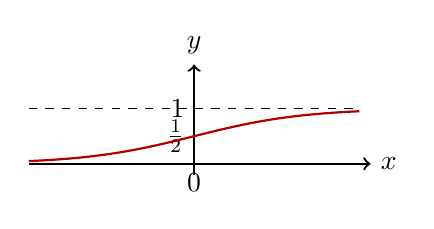
\begin{tikzpicture}[x=0.7cm,y=0.7cm]
    \draw[->, thick] (-3.0,0) -- (3.2,0) node[right] {\(x\)};
    \draw[->, thick] (0,-0.2) -- (0,1.8) node[above] {\(y\)};

    \draw[dashed] (-3,1) -- (3,1);
    \node[left] at (0,1) {\(1\)};
    \node[left] at (0,0.5) {\(\frac{1}{2}\)};

    \draw[thick, red!70!black, domain=-3:3, samples=80]
        plot (\x,{1/(1+exp(-\x))});

    \node[below] at (0,0) {\(0\)};
\end{tikzpicture}
